\documentclass{beamer}
\usepackage[utf8]{inputenc}   % pour pouvoir taper les accents directement
\usepackage[french]{babel}
\usepackage[T1]{fontenc}
\usepackage{amsfonts,amssymb,amsmath}
\usepackage{tikz}
\usepackage{array}
\usepackage{calc}
\usetikzlibrary{patterns}
\usepackage[absolute,showboxes,overlay]{textpos}     
\textblockorigin{0pt}{0pt}                          
\TPshowboxesfalse  
 \usepackage{lmodern,multido}

\newcommand{\R}{\mathbb{R}}
\newcommand{\C}{\mathbb{C}}
\newcommand{\Z}{\mathbb{Z}}
\newcommand{\N}{\mathbb{N}}
\newcommand{\Q}{\mathbb{Q}}

\newcommand{\pop}{\mathcal{U}} % pour ne pas confondre avec la loi de Poisson

\begin{document}
 %%%%%%%%%%%%%%%%%%%%%%%%%%%%%%%%%%%%%%%%%%%%%%%%%%%%%%%%%%%%%%%
 % Afficher le numéro de diapos 
  \addtobeamertemplate{navigation symbols}{}{ \hspace{1em}    \usebeamerfont{footline}%
    \insertframenumber/\inserttotalframenumber }
 %%%%%%%%%%%%%%%%%%%%%%%%%%%%%%%%%%%%%%%%%%%%%%%%%%%%%%%%%%%%%%%

\begin{frame}{Introduction aux statistiques}
\begin{textblock*}{\textwidth}(1cm,2cm)

\begin{center}{\bf \Large Chapitre 4} \end{center}
\begin{center}{\bf \Large Statistique sur moyennes} \end{center}
\vspace{0.5cm}
\begin{itemize}
\item Estimation  
\item Intervalles de confiance
\item Test d'hypothèses 
\end{itemize}
\vspace{0.5cm}
\begin{itemize}
\item Variables quantitatives : moyenne et variance (chapitre 4)
\item Variables qualitatives : proportion (chapitre 5)
\end{itemize}

 \end{textblock*}

\end{frame}


 %%%%%%%%%%%%%%%%%%%%%%%%%%%%%%%%%%%%%%%%%%%%%%%%%%%%%%%%%%%%%%%

\begin{frame}{Estimation}
\begin{textblock*}{\textwidth}(1cm,2cm)

\begin{center}{\bf \Large Problématique} \end{center}

\begin{itemize}
\item Objectif : valeur d'un paramètre $\mu$ associé à une population $\pop$
\vspace{0.5cm}
\begin{itemize}
\item Exemple :  taux d'hémoglobine moyen dans la population humaine
\vspace{0.2cm}
\item Pour connaître la valeur exacte de $\mu$\\

$\rightsquigarrow$ Mesurer le taux d'hémoglobine de chaque individu de $\pop$
\vspace{0.2cm}
\item En pratique \\
$\rightsquigarrow$ Valeur approchée de $\mu$ (estimation) obtenue sur un échantillon tiré au hasard dans $\pop$
\end{itemize}

\end{itemize}

 \end{textblock*}

\end{frame}

 %%%%%%%%%%%%%%%%%%%%%%%%%%%%%%%%%%%%%%%%%%%%%%%%%%%%%%%%%%%%%%%

\begin{frame}{Estimation}
\begin{textblock*}{\textwidth}(1cm,1cm)

\begin{center}{\bf \Large Notations} \end{center}

\begin{itemize}
\item $X : \mathcal{U}\to\R$ variable aléatoire de moyenne $\mu$  et d'écart-type $\sigma$ : c'est la mesure associée à un individu tiré au hasard dans $\pop$

\item $\mathcal{E}_n$ ensemble des échantillons de $n$ individus de $\pop$ 

\item Soit $x=(x_1,\hdots, x_i, \hdots, x_n)$ les valeurs observées sur $n$ individus

	\begin{itemize}
	\item moyenne (empirique) de $x$ :
$\displaystyle \overline{x}=\frac{x_1+\hdots + x_n}{n} = \frac{\sum_{i=1}^n x_i}{n}$
	
	\item variance (empirique) de $x$ :
$\displaystyle  Var(x)=\frac{1}{n} \sum_{i=1}^n (x_i - \overline{x})^2 = \overline{x^2} - \overline{x}^2$
	
	\item écart type (empirique) : $\displaystyle  \sqrt{Var(x)}$ 
	\end{itemize}
\item Modélisation : $x = (x_i)_{1\leq i\leq n}$ est la réalisation de variables aléatoire indépendantes $(X_i)_{1\leq i\leq n}$ toutes de même loi que $X$.
\end{itemize}

%\begin{minipage}{6cm}
%Rappel :
%$\displaystyle Var(x)=\frac{\sum\limits_{k=1}^n x_k^2}{n} - \overline{x}^2$.
%\end{minipage}\ \
%\begin{minipage}{4.5cm}
%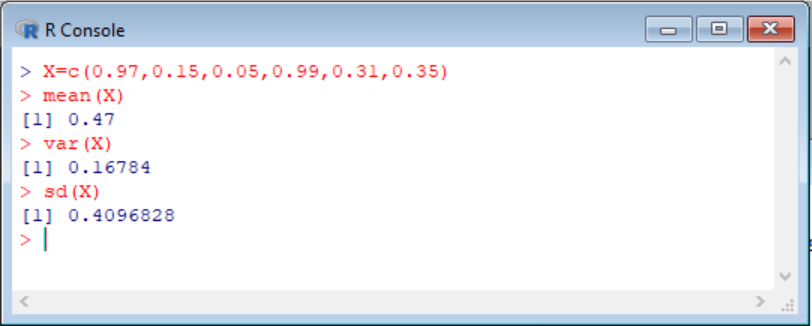
\includegraphics[width=4.5cm]{images/parametres.png}
%\end{minipage}\\ 
\end{textblock*}
\end{frame}
 
 %%%%%%%%%%%%%%%%%%%%%%%%%%%%%%%%%%%%%%%%%%%%%%%%%%%%%%%%%%%%%%%

\begin{frame}{Estimation}
\begin{textblock*}{\textwidth}(1cm,2cm)

\begin{center}{\bf \Large Estimation de moyenne} \end{center}

\begin{itemize}
\item Tirage au hasard dans $\pop$ d'un échantillon de taille $n$
\item Mesures de $X$ sur cet échantillon : $x=(x_1,\hdots, x_n)$
\item Calcul de la moyenne de ces valeurs : $\overline{x}$
\item Estimation de $\mu$ par $\overline{x}$ : la moyenne $\overline{x}$ calculée sur les données de l'échantillon est une estimation de $\mu$ la moyenne inconnue sur la population. 
\item C'est la LGN !
\end{itemize}
%\vspace{0.3cm}
Mais cette estimation n'est pas unique : elle est variable d'un échantillon à l'autre, dans la limite du raisonnable.


 \end{textblock*}

\end{frame}

 
 %%%%%%%%%%%%%%%%%%%%%%%%%%%%%%%%%%%%%%%%%%%%%%%%%%%%%%%%%%%%%%%

\begin{frame}{Estimation}
\begin{textblock*}{\textwidth}(1cm,2cm)

\begin{center}{\bf \Large Estimation de moyenne} \end{center}

Mathématiquement, construction d'une variable aléatoire :

\begin{center}
$M_n : \mathcal{E}_n \longrightarrow \mathbb{R}$  définie par $M_n(echantillon) =  \overline{x} $
\end{center} 
soit 
\[
M_n = \frac{1}{n} (X_1 + \hdots + X_n)=\overline{X}
\]


\begin{itemize}
\item $M_n$ {\bf estimateur} de $\mu$
\item $\overline{x}=$  {\bf une estimation} de $\mu$ = une réalisation de $M_n$
\end{itemize}

\end{textblock*}

\end{frame}

 %%%%%%%%%%%%%%%%%%%%%%%%%%%%%%%%%%%%%%%%%%%%%%%%%%%%%%%%%%%%%%%

\begin{frame}{Estimation}
\begin{textblock*}{\textwidth}(1cm,2cm)

\begin{center}{\bf \Large Estimation de moyenne} \end{center}

\vspace{0.5cm}

$M_n$ est une v.a. définie par : 
\vspace{0.2cm}
\begin{itemize}
\item $E(M_n) = \mu$ : La moyenne de $M_n$ tend vers $\mu$ \\

$\rightsquigarrow$ on dit que l'estimateur $M_n$ est {\bf sans biais} \\
\vspace{0.2cm}
\item $Var(M_n) = \displaystyle \frac{\sigma^2}{n}$ mesure la dispersion des moyennes des échantillons autour de $\mu$ \\

$\rightsquigarrow$ on dit que l'estimateur $M_n$ est {\bf correct} i.e. l'erreur diminue quand la taille de l'échantillon augmente
\end{itemize} 

\end{textblock*}

\end{frame}

 %%%%%%%%%%%%%%%%%%%%%%%%%%%%%%%%%%%%%%%%%%%%%%%%%%%%%%%%%%%%%%%

\begin{frame}{Estimation}
\begin{textblock*}{\textwidth}(1cm,2cm)

\begin{center}{\bf \Large Estimation de moyenne} \end{center}
\vspace{0.5cm}
Quelle est la loi de probabilité de $M_n$ ? 

\
\begin{itemize}
\item Si $n$  grand ($n\geq 30$), on peut appliquer le
Théorème Central Limite :  $M_n\sim \mathcal{N}(\mu ; \sigma/\sqrt{n})$ approximativement

\
\item Si  $n<30$ et $X \sim \mathcal{N}(\mu ; \sigma)$ alors 
$M_n\sim \mathcal{N}(\mu ; \sigma/\sqrt{n})$ exactement

\end{itemize}

\end{textblock*}

\end{frame}

%%%%%%%%%%%%%%%%%%%%%%%%%%%%%%%%%%%%%%%%%%%%%%%%%%%%%%%%%%%%%%

\begin{frame}{Estimation}
\begin{textblock*}{\textwidth}(1cm,1.5cm)

\begin{center}{\bf \Large Estimation de variance} \end{center}

%\vspace{0.5cm}
$V_n : \mathcal{E}_n \longrightarrow \mathbb{R}$ défini par 

\begin{center}
$V_n(echantillon) =  Var(x)=$ variance  de l'échantillon
\end{center}
\vspace{0.3cm}
\begin{itemize}
\item $\displaystyle E(V_n) = \frac{n-1}{n} \sigma^2 \neq \sigma^2$ $\rightsquigarrow$ Problème :  $V_n$ a un biais
\vspace{0.3cm}
\item Solution : $S_n^2=\frac{n}{n-1} V_n$ $\rightsquigarrow$ sans biais \\ \vspace{0.3cm}
C'est un trade-off : la variance corrigée $S_n^2$ varie désormais autour de la bonne valeur, mais elle varie davantage que $V_n$\dots
\end{itemize}
\end{textblock*}

\end{frame}

%%%%%%%%%%%%%%%%%%%%%%%%%%%%%%%%%%%%%%%%%%%%%%%%%%%%%%%%%%%%%%

\begin{frame}{Estimation}
\begin{textblock*}{\textwidth}(1cm,2cm)

\begin{center}{\bf \Large Estimation de variance} \end{center}

\begin{itemize}
\item Estimateur de la variance : 
$$
S^2_n = \frac{1}{n-1} \sum_{i=1}^n (X_i - M_n)^2\,
$$
\item Estimation de $\sigma^2$ sur l'échantillon : 
$$
%S^2_n(echantillon) = 
s^2_x = \frac{1}{n-1} \sum_{i=1}^n (x_i - \overline{x})^2= \frac{1}{n-1}\sum\limits_{i=1}^n x_i^2 - \frac{n}{n-1}\overline{x}^2
$$
\end{itemize}

\end{textblock*}

\end{frame}

 
%%%%%%%%%%%%%%%%%%%%%%%%%%%%%%%%%%%%%%%%%%%%%%%%%%%%%%%%%%%%%%

\begin{frame}{Estimation}
\begin{textblock*}{\textwidth}(1cm,2cm)

\begin{center}{\bf \Large Estimation de variance} \end{center}
\vspace{0.5cm}
\begin{itemize}
\item $E(S^2_n) = \sigma^2$ 
\vspace{0.3cm}
\item la variance de $S_n^2$ tend vers 0 lorsque $n\rightarrow +\infty$
\vspace{0.3cm}
\item $\displaystyle T=\frac{(n-1)S^2_n}{\sigma^2}$ suit approximativement une loi du $\chi^2$ à $n-1$ ddl, si $n$ est assez grand.
\item Seulement si la loi de $X$ est normale, $T$ suit exactement la loi du $\chi^2$ à $n-1$ ddl, même pour $n$ petit.
\end{itemize}


\end{textblock*}

\end{frame}

%%%%%%%%%%%%%%%%%%%%%%%%%%%%%%%%%%%%%%%%%%%%%%%%%%%%%%%%%%%%%%%

\begin{frame}{Intervalle de confiance}
\begin{textblock*}{\textwidth}(1cm,1cm)

\begin{center}{\bf \Large Intervalle de confiance d'une moyenne} \end{center}
\vspace{0.5cm}
On sait que :
$$
M_n\sim \mathcal{N}(\mu ; \sigma/\sqrt{n}) \text{ approximativement}
$$

$$
\Rightarrow \frac{M_n-\mu}{\sigma/\sqrt{n}} \sim \mathcal{N}(0 ; 1)
$$

\begin{itemize}
\item $M_n$ $\rightarrow$ on en connaît une réalisation $\overline{x}$
\item $\mu$ $\rightarrow$ valeur que l'on veut encadrer
\item $\sigma$ $\rightarrow$ inconnu mais on peut utiliser son estimateur $S_n$ dont on connaît une réalisation $s_x$ 
\end{itemize}

\end{textblock*}

\end{frame}

%%%%%%%%%%%%%%%%%%%%%%%%%%%%%%%%%%%%%%%%%%%%%%%%%%%%%%%%%%%%%%%

\begin{frame}{Intervalle de confiance}
\begin{textblock*}{\textwidth}(1cm,1cm)

\begin{center}{\bf \Large Intervalle de confiance d'une moyenne} \end{center}

\vspace{0.2cm}
Dans le cas de {\bf grands échantillons} : \\
$$
T = \frac{M_n-\mu}{S_n/\sqrt{n}} \sim \mathcal{N}(0 ; 1) \text{ approximativement}
$$

%Si $n$ est grand ($n\geq 30$),  $T\sim \mathcal{N}(0;1)$.

$$
\Rightarrow Pr\left(M_n -1.96 \frac{S_n}{\sqrt{n}} \leq \mu \leq M_n + 1.96 \frac{S_n}{\sqrt{n}}\right) \approx 0.95
$$

Sur l'échantillon : 
$$\displaystyle IC_{95\%}(\mu) = \left[\overline{x} - 1.96 \frac{s_x}{\sqrt{n}} ; \overline{x} + 1.96 \frac{s_x}{\sqrt{n}}\right]$$
appelé { \bf intervalle de confiance à $95 \%$ de $\mu$} \\

\end{textblock*}

\end{frame}
 
%%%%%%%%%%%%%%%%%%%%%%%%%%%%%%%%%%%%%%%%%%%%%%%%%%%%%%%%%%%%%%%

\begin{frame}{Intervalle de confiance}
\begin{textblock*}{\textwidth}(1cm,1cm)

\begin{center}{\bf \Large Intervalle de confiance d'une moyenne} \end{center}

Dans le cas de {\bf petits échantillons} : {\bf si  $X\sim \mathcal{N}(\mu ; \sigma)$} alors  

$$\frac{M_n-\mu}{S_n/\sqrt{n}} \sim Student(n-1)$$

L'intervalle de confiance à $95 \%$ de $\mu$  :

\begin{itemize}
\item même forme
\item  on remplace 1.96 par le quantile de la loi de Student (à $n-1$ ddl) pour $\alpha=0.05$ : $t_{(n-1;0.05)}$ à lire dans la table de Student
\end{itemize} 
\vspace{0.2cm}
Sur l'échantillon : 
$$\displaystyle IC_{95\%}(\mu) = \left[\overline{x} - t_{(n-1;0.05)} \frac{s_x}{\sqrt{n}} ; \overline{x} + t_{(n-1;0.05)} \frac{s_x}{\sqrt{n}}\right]$$

\end{textblock*}

\end{frame}
  


%%%%%%%%%%%%%%%%%%%%%%%%%%%%%%%%%%%%%%%%%%%%%%%%%%%%%%%%%%%%%%%

\begin{frame}{Tests statistiques}
\begin{textblock*}{\textwidth}(1cm,2cm)

%\begin{center}{\bf \Large Chapitre 7} \end{center}

\begin{center}{\bf \Large Problématique d'un test statistique} \end{center}
\
\

\begin{itemize}
\item Problème de {\it reproductibilité} des résultats d'une expérience
\vspace{0.2cm}
\item Comparaison de l'efficacité de deux médicaments : effet du hasard/effet du traitement
\vspace{0.2cm}
\item Frontière (probabiliste) permettant d'évaluer si l'écart 
entre les résultats traduit probablement un \og vrai\fg{} phénomène 

\end{itemize}


 \end{textblock*}

\end{frame}



%%%%%%%%%%%%%%%%%%%%%%%%%%%%%%%%%%%%%%%%%%%%%%%%%%%%%%%%%%%%%%%

\begin{frame}{Tests statistiques}
\begin{textblock*}{\textwidth}(1cm,1cm)
\begin{center}{\bf \Large Le choix du test dépend} \end{center}
\vspace{0.2cm}
\begin{itemize}
\item du type de problématique : 
\begin{itemize}
\item  Test de {\it conformité} (avec un échantillon)
\item  Test {\it d'homogénéité} (avec deux échantillons indépendants)
\item  Test avec deux échantillons appariés (non indépendants)
\item  Tests avec plus de deux échantillons
\end{itemize}
\vspace{0.15cm}
\item du type de variables :
\begin{itemize}
\item quantitatives $\rightarrow$ moyennes 
\item qualitatives $\rightarrow$ proportions 
\end{itemize}
\vspace{0.15cm}
\item de la taille de l'échantillon
\vspace{0.15cm}
\item de l'hypothèse alternative testée 
\end{itemize}

\end{textblock*}

\end{frame}

%%%%%%%%%%%%%%%%%%%%%%%%%%%%%%%%%%%%%%%%%%%%%%%%%%%%%%%%%%%%%%%

\begin{frame}{Tests statistiques}
\begin{textblock*}{\textwidth}(1cm,1.5cm)
\begin{center}{\bf \Large Démarche d'un test statistique} \end{center}
\vspace{0.2cm}
\begin{itemize}
\item Quelle est la question posée ? \\
\begin{itemize}
\item Moyennes/Proportions 
\item Grands/petits échantillons  
\item Bi/unilatéral
\end{itemize}
\vspace{0.1cm}
\item Poser les hypothèses $H_0$ et $H_1$ 
\vspace{0.1cm}
\item Poser la statistique de test correspondante. Quelle est sa loi ? \\
En déduire la zone de rejet de $H_0$ 
\vspace{0.1cm}
\item Calculer la statistique de test sur les données de l'échantillon
\vspace{0.1cm}
\item Conclure : Rejet ou non de $H_0$
\end{itemize}

\end{textblock*}

\end{frame}

%%%%%%%%%%%%%%%%%%%%%%%%%%%%%%%%%%%%%%%%%%%%%%%%%%%%%%%%%%%%%%%

\begin{frame}{Test de conformité de moyenne}
\begin{textblock*}{\textwidth}(1cm,1.5cm)

\begin{center}{\bf \Large Test de conformité de moyenne } \end{center}

Données :
\begin{itemize}
\item  moyenne  $m$ obtenue à partir d'un échantillon de taille $n$
\item   valeur théorique connue $\mu_0$
\end{itemize}

\

Problème :

\begin{itemize}
\item différence entre $m$ et $\mu_0$ due au hasard ?
\item différence trop importante :  
l'échantillon n'appartient \emph{probablement} pas à une population de moyenne $\mu_0$.
\item il est significatif de rejeter l'hypothèse $H_0$, généralement pas de l'accepter !
\end{itemize}

\end{textblock*}

\end{frame}
 
 
 %%%%%%%%%%%%%%%%%%%%%%%%%%%%%%%%%%%%%%%%%%%%%%%%%%%%%%%%%%%%%%%

\begin{frame}{Test de conformité de moyenne}
\begin{textblock*}{\textwidth}(1cm,2cm)

\begin{center}{\bf \Large Exemple } \end{center}


\begin{itemize}
\item fouines en conditions naturelles : durée de vie $\mu_0\approx 12$ ans.
\item fouines en milieu urbain : durée de vie  impactée ?
\end{itemize}

\

Données : 84 fouines citadines suivies jusqu'à leur mort. 
\begin{itemize}
\item durées de vie $x_1\,\hdots,x_{84}$
\item moyenne $m = \overline{x} \approx 11.1$
\item écart-type empirique $s_x\approx 2.9$
\end{itemize}

\end{textblock*}

\end{frame}

%%%%%%%%%%%%%%%%%%%%%%%%%%%%%%%%%%%%%%%%%%%%%%%%%%%%%%%%%%%%%%%

\begin{frame}{Test de conformité de moyenne}
\begin{textblock*}{\textwidth}(1cm,1.3cm)

\begin{center}{\bf \Large Exemple } \end{center}

\begin{itemize}
\item  $X$ v.a. = durée de vie des fouines  citadines 
\item $X$ de moyenne $\mu$ et de variance $\sigma^2$  inconnues. 
\item  $M_n$ et $S^2_n$ les estimateurs de $\mu$ et de $\sigma^2$ pour des échantillons de taille $n$ (ici $n=84$)\\
\end{itemize}

\

{\bf Formulation des hypothèses nulle et alternative}

\begin{itemize}
\item $H_0 : \mu=\mu_0$ : pas de différence de durée de vie entre les fouines citadines et campagnardes
\item $H_1 : \mu \neq \mu_0$ : différence de durée de vie entre les fouines citadines et campagnardes \\
$\rightarrow H1$ = conclusion du test si on rejette $(H_0)$ 
\end{itemize}


\end{textblock*}

\end{frame}
 
 %%%%%%%%%%%%%%%%%%%%%%%%%%%%%%%%%%%%%%%%%%%%%%%%%%%%%%%%%%%%%%%

\begin{frame}{Test de conformité de moyenne}
\begin{textblock*}{\textwidth}(1cm,2cm)

\begin{center}{\bf \Large Statistique de test} \end{center}

\

Dans le cas de grands échantillons, on a vu que : \\
$$
T = \frac{M_n-\mu}{S_n/\sqrt{n}} \sim \mathcal{N}(0 ; 1)
$$

\

On pose la {\bf statistique de test} sous $H_0$

$$T=\frac{M_n-{\color{red} \mu_0}}{S_n/\sqrt{n}} \sim \mathcal{N}(0,1)$$ 

Sous $H_0$ : $\displaystyle T \sim \mathcal{N}(0,1) \; \Rightarrow \; \Pr(-z_{\alpha}<T<z_{\alpha}) = 1-\alpha$

\end{textblock*}

\end{frame}
%%%%%%%%%%%%%%%%%%%%%%%%%%%%%%%%%%%%%%%%%%%%%%%%%%%%%%%%%%%%%%%

\begin{frame}{Test de conformité de moyenne}
\begin{textblock*}{\textwidth}(1cm,1.5cm)

\begin{center}{\bf \Large Zone de rejet de $H_0$} \end{center}

On fixe le risque de 1ère espèce : $\alpha\in{} ]0,1[$ (en général $0.05$) 
$$
\alpha = \Pr(Rejeter \; H_0 / H_0 \; vraie)
$$

\begin{center}
\begin{tikzpicture}[xscale=2,yscale=1.8]
\draw[->] (-0.1,0) -- (3,0);
\draw (0.4,-0.2) node {$-z_\alpha$};
\draw (1.8,-0.2) node {$z_\alpha$};
\draw[color=red](2.5,0.2) node {$\Pr(T>z_{\alpha}) = \alpha/2$};
\draw[color=red](-0.5,0.2) node {$\Pr(T<-z_{\alpha}) = \alpha/2$};
\draw (1.1,-0.5) node {Z.A. de $H_0$};
\draw[color=red](2.4,-0.5) node {Z.R. de $H_0$};
\draw[color=red](-0.2,-0.5) node {Z.R. de $H_0$};
\draw (2,1.4) node {Loi de $T$ sous $H_0$};
\draw plot file {data/densite_norm_5.txt};
\fill[color=red] plot file {data/densite_norm_5.txt};
\draw plot file {data/densite_norm_95.txt} -- cycle;
\fill[color=white] plot file {data/densite_norm_95.txt} -- cycle;
\draw[->] (1,-0.05) -- (1,1.4);
\end{tikzpicture}
\end{center}
\end{textblock*}

\end{frame}

%%%%%%%%%%%%%%%%%%%%%%%%%%%%%%%%%%%%%%%%%%%%%%%%%%%%%%%%%%%%%%%

\begin{frame}{Test de conformité de moyenne}
\begin{textblock*}{\textwidth}(1cm,1.5cm)

\begin{center}{\bf \Large Règle de décision} \end{center}

\begin{center}{avec $\alpha = 0.05$} \end{center}

\
\begin{itemize}
\item Si $|t| > 1.96 \; \Rightarrow \; $ Rejet de $H_0$ \\

$\rightsquigarrow$ Mise en évidence d'une différence significative entre $m$ et $\mu_0$ \\
$\rightsquigarrow$ Il est crédible que $\mu\neq\mu_0$

\
\item Si $|t| < 1.96 \; \Rightarrow \; $ Non-rejet de $H_0$ \\

$\rightsquigarrow$ Pas de différence significative entre $m$ et $\mu_0$ \\
$\rightsquigarrow$ On ne peut pas exclure que $\mu = \mu_0$

\end{itemize}

\end{textblock*}

\end{frame}


%%%%%%%%%%%%%%%%%%%%%%%%%%%%%%%%%%%%%%%%%%%%%%%%%%%%%%%%%%%%%%%

\begin{frame}{Test de conformité de moyenne}
\begin{textblock*}{\textwidth}(1cm,1.5cm)

\begin{center}{\bf \Large Mise en œuvre} \end{center}

\begin{itemize}
\item $\alpha$ fixé à 0.05 
\item Valeur seuil correspondante pour $\mathcal{N}(0,1)$ : 1.96
\item Sous $H_0$ : $\mu=\mu_0=12$
\item On calcule :
$$t=\frac{m-\mu_0}{\frac{s_x}{\sqrt{n}}} \approx -2.844$$
\item  $|t|>1.96$ donc on rejette l'hypothèse $H_0$
\end{itemize}

Si $H_0$ était effectivement vraie, il y aurait moins de 5\% de chances qu'une telle valeur de la durée de vie (sur un échantillon de taille 84) soit au moins aussi éloignée de la valeur moyenne dans la population

\end{textblock*}

\end{frame}

%%%%%%%%%%%%%%%%%%%%%%%%%%%%%%%%%%%%%%%%%%%%%%%%%%%%%%%%%%%%%%%

\begin{frame}{Test  de conformité de moyenne}
\begin{textblock*}{\textwidth}(1cm,2cm)

\begin{center}{\bf \Large Conclusion  } \end{center}

\

Au risque de 5\%, on conclut que $\mu\neq\mu_0$, il y a une différence significative entre les durées de vie moyennes

\

Or $m<\mu_0$, on peut raisonnablement conclure
(peut-être à tort mais on prend le risque) que la vie citadine diminue l'espérance de vie des fouines

\end{textblock*}

\end{frame}

%%%%%%%%%%%%%%%%%%%%%%%%%%%%%%%%%%%%%%%%%%%%%%%%%%%%%%%%%%%%%%%%%%


\begin{frame}{Test de conformité de moyenne}
\begin{textblock*}{\textwidth}(1cm,1.5cm)

\begin{center}{\bf \Large Degré de signification  } \end{center}

\vspace{0.5cm}

{\bf Degré de signification} = plus petit $\epsilon$ tel que $|t|>z_\epsilon$ 

 \
\begin{columns}[c]
  \begin{column}{6cm}
A partir de la table des valeurs extrêmes de $N(0,1)$  \\
Si on avait pris $\epsilon$ au lieu de $\alpha$ comme risque d'erreur, $H_0$ encore rejetée mais avec probabilité $\epsilon<\alpha$ de se tromper
  \end{column}
  \begin{column}{4cm}
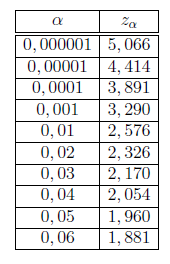
\includegraphics[scale=0.6]{images/g_degredesignification.png}
  \end{column}
 \end{columns}  

Exemple : $ t=-2.84 \; \Rightarrow \; \epsilon<0.01 $ (mais $\epsilon > 0.001$).

\end{textblock*}

\end{frame}

%%%%%%%%%%%%%%%%%%%%%%%%%%%%%%%%%%%%%%%%%%%%%%%%%%%%%%%%%%%%%%%%%



\begin{frame}{Test de conformité de moyenne }
\begin{textblock*}{\textwidth}(1cm,1.5cm)

\begin{center}{\bf \Large Remarques} \end{center}

\begin{itemize}
\item  Conclusion si $|t| < 1.96$ ?
 
Les données ne permettent pas de rejeter $H_0$. 
Mais on n'accepte pas $H_0$ ! {\bf Ne jamais dire : \og rejeter $H_1$\fg}\\
Si on sélectionne $H_0$, c'est seulement par défaut, car rien ne garantit que $H_0$ est vraie \\
$\rightarrow$ La théorie des tests statistiques a été pensée pour rejeter des hypothèses

\vspace{0.2cm}
\item 1.96 {\it seuil critique} associé au risque d'erreur 0.05

Avec des valeurs plus petites de $\alpha$ : on diminue le risque de se tromper (lorsque $H_0$ est vraie) mais on rejette moins souvent $H_0$ (y compris lorsqu'elle est fausse)

\end{itemize} 

\end{textblock*}
\end{frame}

%%%%%%%%%%%%%%%%%%%%%%%%%%%%%%%%%%%%%%%%%%%%%%%%%%%%%%%%%%%%%%%%%



\begin{frame}{Test de conformité de moyenne }
\begin{textblock*}{\textwidth}(1cm,2cm)

\begin{center}{\bf \Large Cas des petits échantillons} \end{center}

\begin{itemize}
\item Si $X$ {\it suit une loi normale}, on a vu que : 

$$T = \frac{M_n-\mu}{S_n/\sqrt{n}} \sim Student(n-1)$$

\

\item Même démarche mais on compare $t$ à la valeur seuil de la loi de Student à $n-1$ ddl pour $\alpha=0.05$  

\ 

\item Exemple : si $n=15$, le seuil critique pour $\alpha = 0.05$ est $t_{(14;0.05)}=2.145$ 
\end{itemize} 


%\begin{center}
%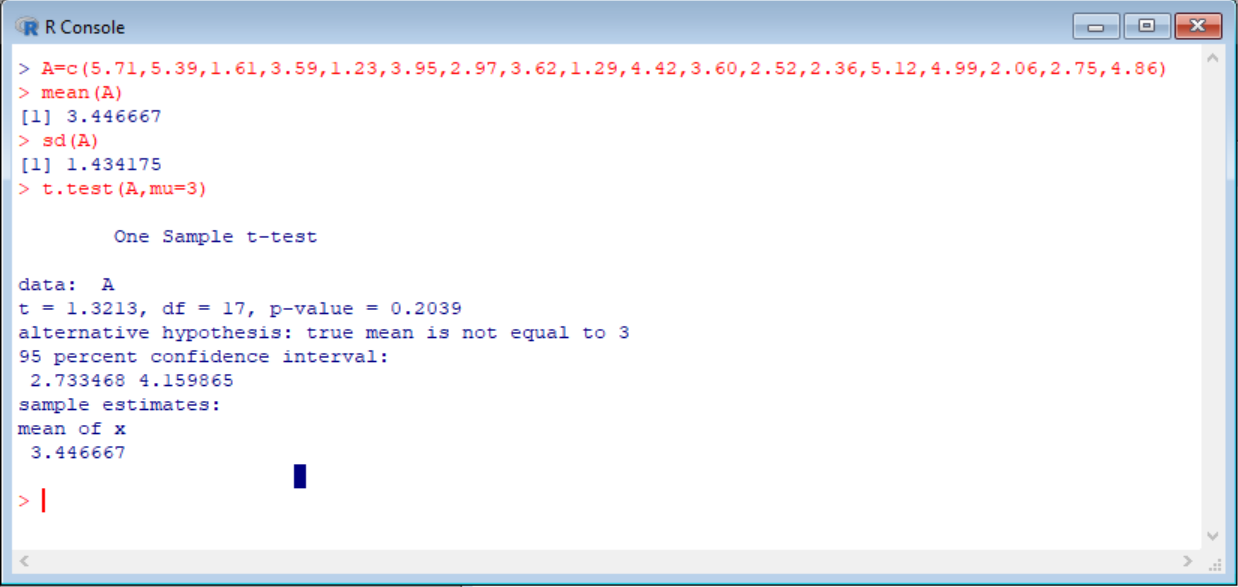
\includegraphics[width=5cm]{images/conformite_moyenne_student.png}
%\end{center}

\end{textblock*}
\end{frame}

%%%%%%%%%%%%%%%%%%%%%%%%%%%%%%%%%%%%%%%%%%%%%%%%%%%%%%%%%%%%%%%

\begin{frame}{Test de conformité de moyenne}
\begin{textblock*}{\textwidth}(1cm,2cm)

\begin{center}{\bf \Large  Tests unilatéraux  } \end{center}


Exemple :
\begin{itemize}
\item  $X$ la variable aléatoire = temps de guérison de la migraine
\item Le temps ne peut qu'être diminué par le traitement
\end{itemize}

\

{\bf Formulation des hypothèses nulle et alternative }

\begin{itemize}
\item $H_0 : \mu=\mu_0$ : pas de différence de temps de guérison
\item $H_1 : \mu <\mu_0$ : le remède diminue le temps de guérison 
\end{itemize}


\end{textblock*}

\end{frame}
 


%%%%%%%%%%%%%%%%%%%%%%%%%%%%%%%%%%%%%%%%%%%%%%%%%%%%%%%%%%%%%%%

\begin{frame}{Test de conformité de moyenne}
\begin{textblock*}{\textwidth}(1cm,1.5cm)

\begin{center}{\bf \Large Test unilatéraux } \end{center}

La zone de rejet n'est pas divisée en deux parties symétriques mais
concentrée sur un côté \; $\rightarrow$ \; $\mu>\mu_0$ pas envisageable \\

\ 

 $\rightsquigarrow$ Zone de rejet sur la partie négative de la courbe

\begin{center}
\begin{tikzpicture}[xscale=2,yscale=1.8]
\draw[->] (-0.1,0) -- (3,0);
\draw (0.5,-0.2) node {$-z_\alpha$};
\draw[color=red](-0.5,0.2) node {$\Pr(T<-z_{\alpha}) = \alpha$};
\draw (1.5,-0.5) node {Z.A. de $H_0$};
\draw[color=red](0,-0.5) node {Z.R. de $H_0$};
\draw plot file {data/densite_norm_5.txt};
\fill[color=red] plot file {data/densite_norm_5.txt};
\draw plot file {data/densite_norm_95_uni.txt} -- cycle;
\fill[color=white] plot file {data/densite_norm_95_uni.txt} -- cycle;
\draw[->] (1,-0.05) -- (1,1.4);
\end{tikzpicture}
\end{center}
\end{textblock*}

\end{frame}

%%%%%%%%%%%%%%%%%%%%%%%%%%%%%%%%%%%%%%%%%%%%%%%%%%%%%%%%%%%%%%%



\begin{frame}{Test de conformité de moyenne}
\begin{textblock*}{\textwidth}(1cm,2cm)

\begin{center}{\bf \Large Test unilatéraux  } \end{center}

\begin{itemize}
\item Grands échantillons : loi normale centrée réduite 
$$\Pr(T<-1.65)=0.05$$

\item Petits échantillons : loi de Student 
$$
Pr(T<-t_{(n-1;0.10)})=0.05
$$
\emph{à condition qu'on puisse justifier la gaussianité des données}
\end{itemize}

%\begin{center}
%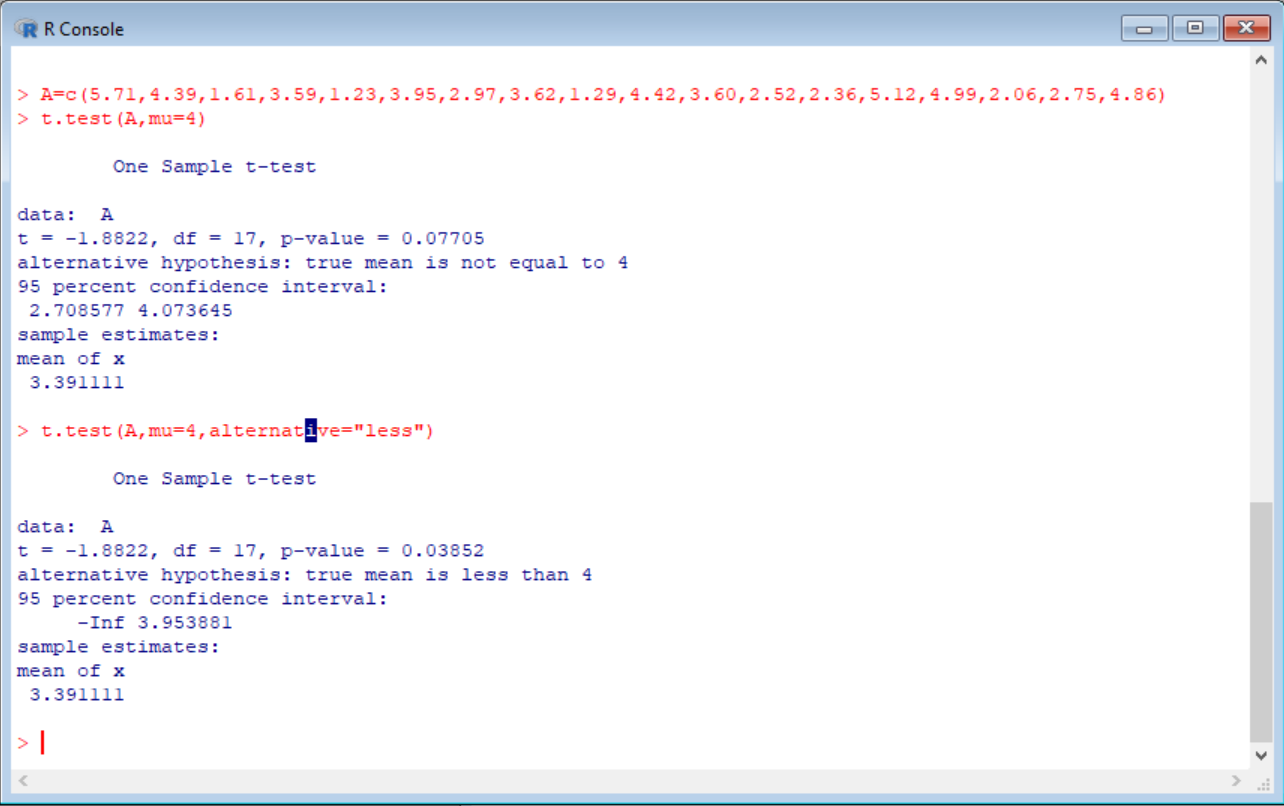
\includegraphics[width=6cm]{images/conformite_moyenne_uni.png}
%\end{center}


\end{textblock*}
\end{frame}


%%%%%%%%%%%%%%%%%%%%%%%%%%%%%%%%%%%%%%%%%%%%%%%%%%%%%%%%%%%%%%%

\begin{frame}{Test d'homogénéité de moyennes}
\begin{textblock*}{\textwidth}(1cm,2cm)

\begin{center}{\bf \Large Test d'homogénéité de moyennes } \end{center}

\

\begin{itemize}
\item Deux échantillons {\it indépendants} issus de deux populations
\item Deux moyennes $m_1$ et $m_2$ différentes
\item La différence entre $m_1$ et $m_2$ se généralise-t-elle aux populations ?
\end{itemize}

\end{textblock*}
\end{frame}

%%%%%%%%%%%%%%%%%%%%%%%%%%%%%%%%%%%%%%%%%%%%%%%%%%%%%%%%%%%%%%%

\begin{frame}{Test d'homogénéité de moyennes}
\begin{textblock*}{\textwidth}(1cm,2cm)

\begin{center}{\bf \Large Exemple } \end{center}
\

\begin{itemize}
\item 50 étudiants (au hasard)   : une portion de 
camembert à chaque repas pendant toute l'année 

notes en mathématiques : $m_1\approx 9.1$ et  $s_1\approx 1.2$

\

\item  60 étudiants (au hasard) : jamais de 
camembert 

notes en Mathématiques : $m_2\approx 8.7$ et $s_2\approx 1.5$

\

\item Influence de la consommation de camembert sur les résultats en mathématiques  ?
\end{itemize}

\end{textblock*}
\end{frame}

%%%%%%%%%%%%%%%%%%%%%%%%%%%%%%%%%%%%%%%%%%%%%%%%%%%%%%%%%%%%%%%

\begin{frame}{Test d'homogénéité de moyennes}
\begin{textblock*}{\textwidth}(1cm,1.5cm)

\begin{center}{\bf \Large Exemple } \end{center}


\

\begin{itemize}
\item $M_1$ et $S_1$ estimateur de $\mu_1$ et $\sigma_1$ sur des éch. de taille $n_1=50$
\item $M_2$ et $S_2$ estimateur de $\mu_2$ et $\sigma_2$ sur des éch. de taille $n_2=60$
\item Echantillons indépendants $\rightarrow$ Variables aléatoires $M_1$ et $M_2$ indépendantes
\end{itemize}

\

{\bf Hypothèses nulle et alternative :}

\begin{itemize}
\item $H_0 : \mu_1=\mu_2$ : le camembert n'a aucune influence
\item  $H_1 : \mu_1\neq\mu_2$
\end{itemize}

\end{textblock*}
\end{frame}


%%%%%%%%%%%%%%%%%%%%%%%%%%%%%%%%%%%%%%%%%%%%%%%%%%%%%%%%%%%%%%%

\begin{frame}{Test d'homogénéité de moyennes}
\begin{textblock*}{\textwidth}(1cm,1.5cm)

\begin{center}{\bf \Large Grands échantillons} \end{center}
\vspace{0.2cm}
\begin{itemize}
\item Statistique de test sous $H_0$ : $
\displaystyle T=\frac{M_1-M_2}{\sqrt{\frac{S_1^2}{n_1}+\frac{S_2^2}{n_2}} }
$
\item $n_1$ et $n_2$  grands : $T\sim \mathcal{N}(0,1)$ approximativement \\ (en pratique on demande $n_1$ et $n_2$ supérieurs à 30)

\
\item Règle de décision : 
\begin{itemize}
\item Si $|t| > z_{\alpha} \; \Rightarrow \; $ Rejet de $H_0$ (au taux d'erreur $\alpha$) \\
$\rightsquigarrow$ Différence \emph{significative} entre les moyennes observées \\
$\rightsquigarrow$ Mise en évidence d'une différence entre $\mu_1$ et $\mu_2$ \\

\
\item Si $|t| < z_{\alpha} \; \Rightarrow \; $ Non-rejet de $H_0$ \\

$\rightsquigarrow$ Pas de mise en évidence d'une différence entre $\mu_1$ et $\mu_2$

\end{itemize}
\end{itemize}

\end{textblock*}
\end{frame}

%%%%%%%%%%%%%%%%%%%%%%%%%%%%%%%%%%%%%%%%%%%%%%%%%%%%%%%%%%%%%%%

\begin{frame}{Test d'homogénéité de moyennes}
\begin{textblock*}{\textwidth}(1cm,2cm)

\begin{center}{\bf \Large Mise en œuvre} \end{center}

\
\begin{itemize}
\item Calcul de $t$ sur les données des 2 échantillons :
$$t= \frac{m_1-m_2}{\sqrt{\frac{s_1^2}{n_1}+\frac{s_2^2}{n_2}} } \approx 1.55 $$

\
\item On fixe $\alpha=0.05$ ; $\Pr(|T|>1.96)=0.05$

\
\item Conclusion :  $|t|<1.96$, on ne peut pas rejeter $H_0$
\end{itemize}

\end{textblock*}
\end{frame}

%%%%%%%%%%%%%%%%%%%%%%%%%%%%%%%%%%%%%%%%%%%%%%%%%%%%%%%%%%%%%%%

\begin{frame}{Test d'homogénéité de moyennes}
\begin{textblock*}{\textwidth}(1cm,1.5cm)

\begin{center}{\bf \Large Petits échantillons } \end{center}

\vspace{0.2cm}

\begin{itemize}
\item $X_1$ (resp. $X_2$) note de maths d'un étudiant de la première (resp. deuxième) population de moyenne $\mu_1$ (resp. $\mu_2$)
\item Uniquement si $X_1$ et $X_2$ sont de lois normales
\item On suppose en outre que $\sigma_1=\sigma_2$
\item on pose la statistique de test sous $H_0$ : 
$$T=\frac{M_1-M_2}{\sqrt{\frac{S^2}{n_1}+\frac{S^2}{n_2}} } \; \sim \; Student(n_1+n_2-2)$$ 
\end{itemize}
avec $\displaystyle S^2=\frac{(n_1-1)S_1^2+(n_2-1)S_2^2}{n_1 + n_2-2} $ estimateur de variance commune
\end{textblock*}
\end{frame}

%%%%%%%%%%%%%%%%%%%%%%%%%%%%%%%%%%%%%%%%%%%%%%%%%%%%%%%%%%%%%%%

\begin{frame}{Test d'homogénéité de moyennes}
\begin{textblock*}{\textwidth}(1cm,1.5cm)

\begin{center}{\bf \Large Petits échantillons } \end{center}

\vspace{0.2cm}
\begin{itemize}
\item Calcul  de $\displaystyle s^2=\frac{(n_1-1)s_1^2+(n_2-1)s_2^2}{n_1+n_2-2}$

\
\item Calcul de $\displaystyle t= \frac{m_1-m_2}{\sqrt{\frac{s^2}{n_1}+\frac{s^2}{n_2}} }$

\
\item Comparaison de $|t|$ avec le seuil critique déterminé par la loi de Student $t_{(n_1+n_2-2;\alpha)}$ 

\
\item Régle de décision :
\begin{itemize}
\item Si $|t| > t_{(n_1+n_2-2;\alpha)} \; \Rightarrow \; $ Rejet de $H_0$
\item Si $|t| < t_{(n_1+n_2-2;\alpha)} \; \Rightarrow \; $ Non-rejet de $H_0$
\end{itemize}

\end{itemize}

\end{textblock*}
\end{frame}



%%%%%%%%%%%%%%%%%%%%%%%%%%%%%%%%%%%%%%%%%%%%%%%%%%%%%%%%%%%%%%%

\begin{frame}{Test d'homogénéité de moyennes}
\begin{textblock*}{\textwidth}(1cm,2cm)

\begin{center}{\bf \Large Petits échantillons } \end{center}



%\begin{center}
%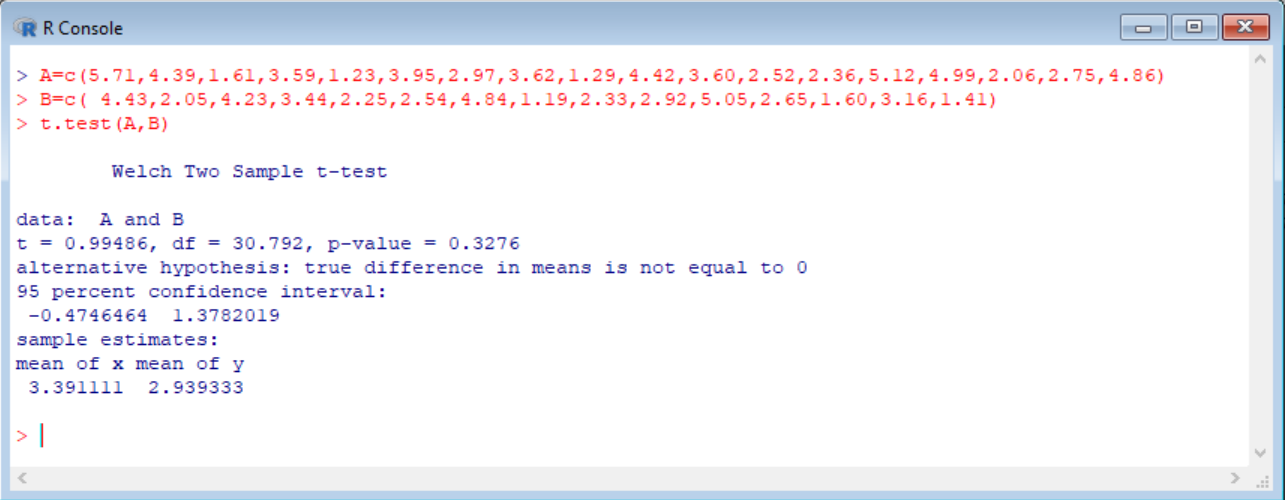
\includegraphics[width=6cm]{images/homogeneite_moyenne.png}
%\end{center}

Problème des hypothèses supplémentaires 

\begin{itemize}
\item Distribution normale : test de {\it Shapiro-Wilk}, de {\it Bontemps Meddahi}, du $\chi^2$
\item Egalité des variances : test de {\it Fisher-Snedecor} (ou "test F") 
\item Ce ne sont pas des garanties ! \\
Cela permet juste d'éliminer \emph{a posteriori} des situations où les hypothèses ne sont vraiment pas légitimes
\item Mais comme les échantillons sont justement petits, il y a peu de chances que les tests servent à quoi que ce soit\dots
\end{itemize}

\end{textblock*}
\end{frame}


%%%%%%%%%%%%%%%%%%%%%%%%%%%%%%%%%%%%%%%%%%%%%
\end{document}




 








